
\section{Task 1: Stride Pattern Prefetching}

\subsection{Task 1A: IP-stride prefetcher}
The provided IP-stride prefetcher (\texttt{ip\_stride.l1d\_pref}) keeps 24 trackers, fully associative with LRU replacement, indexed by the low 8 bits of the load IP.
Each tracker stores the last cache-line address seen from that IP and the last stride.
A new IP allocates a tracker and prefetches nothing.
On a repeat access the line stride is computed and a zero stride is ignored.
If the stride equals the stored one, the next 3 lines (degree 3) at multiples of the stride are prefetched, stopping at the 4~KB page boundary.
The fill level is L1 while the MSHR is under half full, otherwise L2.
The tracker is then updated with the new address and stride.
Because it remembers a single stride and needs it to repeat, an IP that cycles through $(+1,+2,+2,+2,+3)$ rarely has two equal consecutive strides at the right moment and gets few useful prefetches.
The 8-bit IP mask also lets different IPs alias onto one tracker.

\subsection{Task 1B: SPP design}
\paragraph{Tables.}
(1) An IP table of 64 direct-mapped entries holds per-IP last offset, last stride, a confidence counter, a uniform-mode bit and a 12-bit stride signature.
(2) A pattern table of 256 entries, shared across IPs and indexed by a hash of the signature, holds the next stride that followed that signature and a 2-bit confidence.
(3) A 128-entry recent-prefetch filter of partial line tags is filled when a prefetched line arrives in L1D and counts demand hits on prefetched lines.
(4) A 256-entry resident filter approximates which lines are in L1D (set on hits, fills and issued prefetches, cleared on evictions) and is used to skip redundant prefetches.

\paragraph{Dual pattern classification.}
An IP enters uniform mode after the same stride is seen four times in a row (confidence saturates at 3) and leaves it when confidence falls to 1 or below.
In uniform mode it prefetches $s, 2s, \dots$ up to the current degree.
Otherwise every observed stride trains the pattern table under the previous signature,
$\mathrm{sig}' = ((\mathrm{sig} \ll 3)\oplus s)\ \&\ \mathtt{0xFFF}$,
and prediction walks the table from the current signature, feeding each predicted stride back into the signature, up to the current degree.
The walk stops at the first entry with zero confidence.
Requiring four equal strides for uniform mode prevents a run of three $+2$ strides inside $(+1,+2,+2,+2,+3)$ from being mistaken for a uniform stream.
Every prefetch offset is checked to lie inside the current 4~KB page.

\subsection{Storage overhead}
\begin{center}
\small
\begin{tabular}{lrrp{5.0cm}p{2.3cm}}
\toprule
Structure & Entries & Bits/entry & Fields & Total bits \\
\midrule
IP table & 64 & 45 & valid 1, uniform 1, conf 2, tag 8, page hash 8, last offset 6, last stride 7, signature 12 & 2880 \\
Pattern table & 256 & 9 & next stride 7, conf 2 & 2304 \\
Recent-prefetch filter & 128 & 10 & valid 1, partial tag 9 & 1280 \\
Resident filter & 256 & 9 & valid 1, partial tag 8 & 2304 \\
Accuracy counters & 1 & 18 & prefetch fills 7, useful 9, degree 2 & 18 \\
Total &  &  &  & 8786 bits (1098.3 bytes) \\
\bottomrule
\end{tabular}
\end{center}
Without the resident filter the total is 6482 bits.

\subsection{Accuracy-based throttling}
Every 64 prefetch fills into L1D the accuracy (useful fills divided by fills) is evaluated and the degree is set to 1 below $T_1$\%, 2 below $T_2$\%, 3 below $T_3$\% and 4 otherwise.
We swept five threshold sets and three fixed degrees over the three traces:
\begin{center}
\small
\begin{tabular}{lrrrr}
\toprule
Variant & Geomean speedup & Mean accuracy \% & Mean coverage \% & Epochs at degree 1/2/3/4 \\
\midrule
spp\_d1 & 1.0099 & 40.2 & 7.4 & 4600/0/0/0 \\
spp\_d2 & 1.0100 & 34.2 & 8.9 & 0/6823/0/0 \\
spp\_d4 & 1.0090 & 28.6 & 9.7 & 0/0/0/9143 \\
spp\_norf & 1.0120 & 39.7 & 9.5 & 2201/1434/995/1280 \\
spp\_t20\_40\_60 & 1.0121 & 38.1 & 9.8 & 1665/1478/1249/1992 \\
spp\_t25\_50\_75 & 1.0120 & 38.9 & 9.5 & 1922/1543/1363/1270 \\
spp\_t30\_55\_75 & 1.0120 & 39.4 & 9.3 & 2178/1471/992/1284 \\
spp\_t40\_60\_80 & 1.0119 & 39.9 & 9.0 & 2602/1081/990/1028 \\
spp\_t50\_70\_90 & 1.0116 & 40.3 & 8.7 & 2928/999/921/627 \\
\bottomrule
\end{tabular}
\end{center}
% EDIT: confirm these statements against your sweep table before submitting.
Throttled variants (1.0116 to 1.0121 geomean speedup) beat every fixed degree (1.0090 to 1.0100).
Fixed degree 4 has the highest coverage but the lowest accuracy and speedup, consistent with cache pollution; the throttle recovers the benefit of a high degree without it.
The threshold sets differ by only about 0.05\%, so performance is insensitive to their exact values.
We keep 30/55/75, within 0.01\% of the best speedup with moderate accuracy.
The maximum degree of 4 keeps a single trigger from filling more than half of the 8-entry prefetch queue, and the degree never drops to 0 so accuracy remains measurable.

\paragraph{Resident filter.}
Without it SPP issues 763K, 452K and 3.49M prefetch requests on the three traces; with it 263K, 132K and 469K.
Useful prefetches, prefetches sent to the lower level and IPC (1.0120 both ways) are unchanged.
The filter costs 2304 bits and reduces L1D prefetch traffic rather than improving speedup.

\subsection{Results}
\subsection*{IP-stride}
\begin{center}
\small
\begin{tabular}{lrrrrr}
\toprule
Trace & IPC & Speedup & L1D load MPKI & Accuracy (\%) & Coverage (\%) \\
\midrule
Trace1-001\_ & 0.233 & 1.005 & 10.12 & 64.9 & 5.2 \\
Trace2-002\_ & 0.251 & 1.000 & 13.44 & 40.9 & 0.7 \\
Trace3-002\_ & 0.383 & 1.002 & 3.32 & 20.5 & 2.5 \\
Geomean / mean & 0.282 & 1.002 & 8.96 & 42.1 & 2.8 \\
\bottomrule
\end{tabular}
\end{center}
\subsection*{SPP}
\begin{center}
\small
\begin{tabular}{lrrrrr}
\toprule
Trace & IPC & Speedup & L1D load MPKI & Accuracy (\%) & Coverage (\%) \\
\midrule
Trace1-001\_ & 0.233 & 1.005 & 9.73 & 44.8 & 8.9 \\
Trace2-002\_ & 0.253 & 1.008 & 13.19 & 31.2 & 2.6 \\
Trace3-002\_ & 0.391 & 1.023 & 2.84 & 42.1 & 16.6 \\
Geomean / mean & 0.285 & 1.012 & 8.59 & 39.4 & 9.3 \\
\bottomrule
\end{tabular}
\end{center}
Accuracy is the simulator's useful over useful-plus-useless prefetched lines. Coverage is the reduction in L1D load misses relative to the no-prefetching baseline.
% EDIT: add the simulator's own ACCURACY line (useful / issued to lower level) as a second column if you report both.
SPP improves on IP-stride in speedup and coverage, but IP-stride has higher accuracy on two traces because it issues far fewer prefetches.
All three traces are dominated by L2 and LLC misses (baseline LLC load MPKI 12.3, 8.2 and 3.1), which limits what an L1D prefetcher can gain.
\begin{figure}[h]
\centering
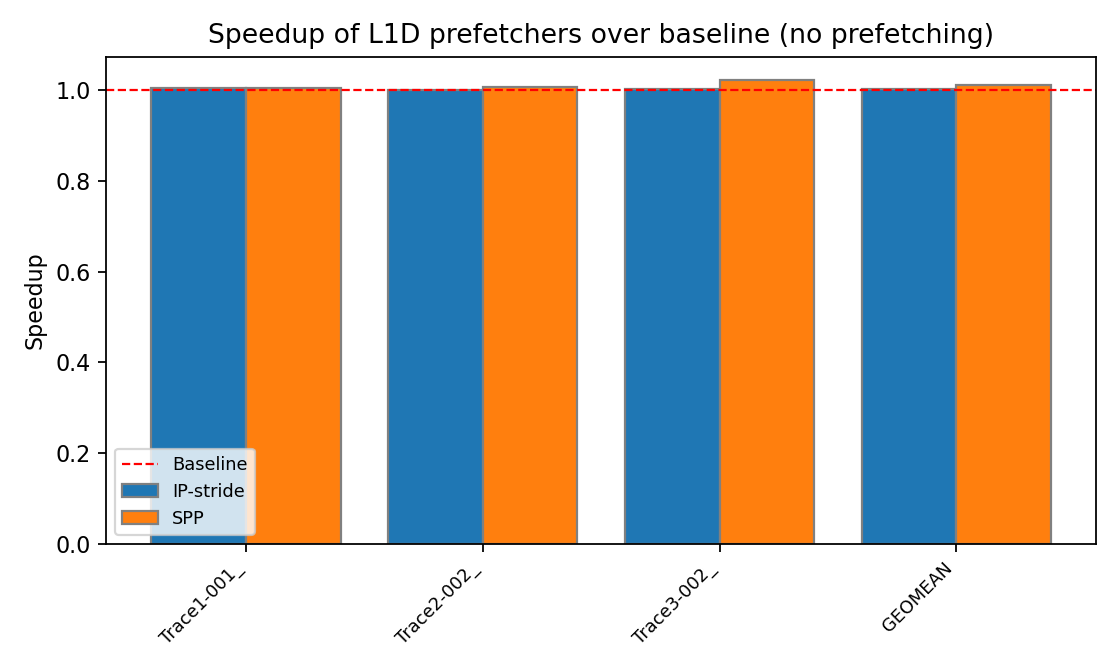
\includegraphics[width=0.8\linewidth]{../plots/task1/speedup.png}
\caption{Speedup over the no-prefetching baseline.}
\end{figure}\begin{figure}[h]
\centering
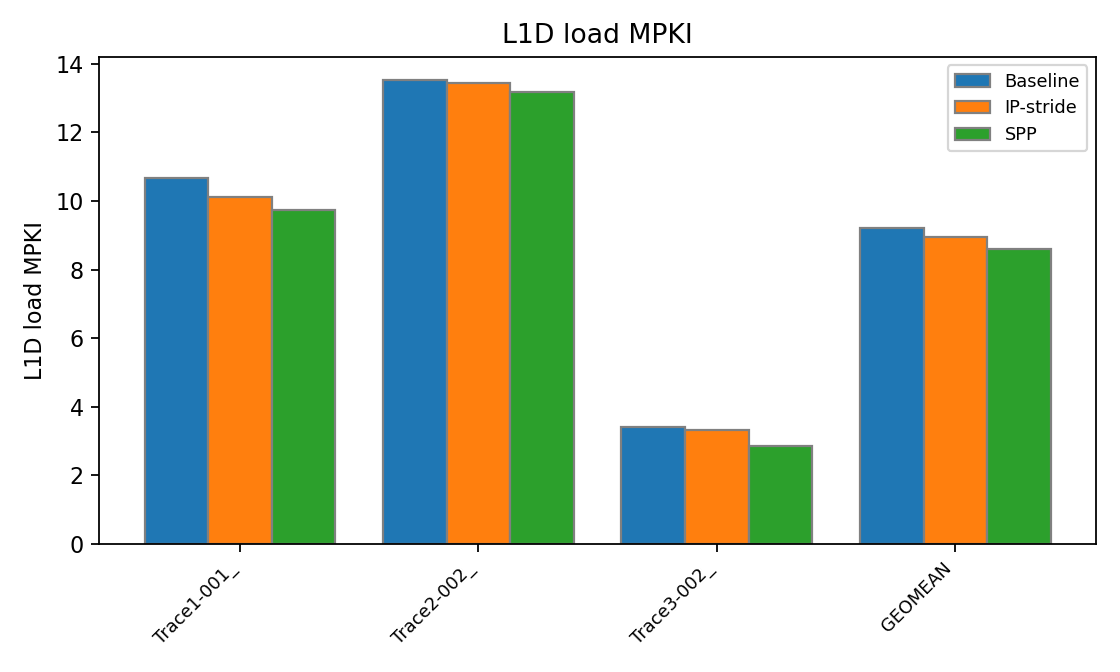
\includegraphics[width=0.8\linewidth]{../plots/task1/mpki.png}
\caption{L1D load MPKI.}
\end{figure}\begin{figure}[h]
\centering
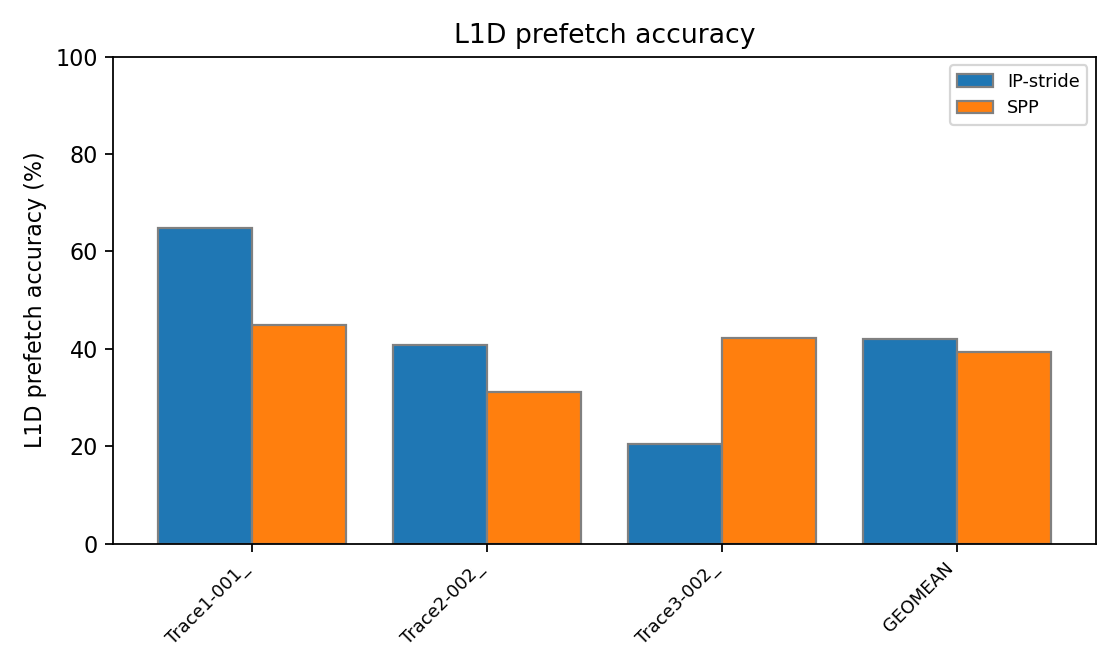
\includegraphics[width=0.8\linewidth]{../plots/task1/accuracy.png}
\caption{L1D prefetch accuracy.}
\end{figure}\begin{figure}[h]
\centering
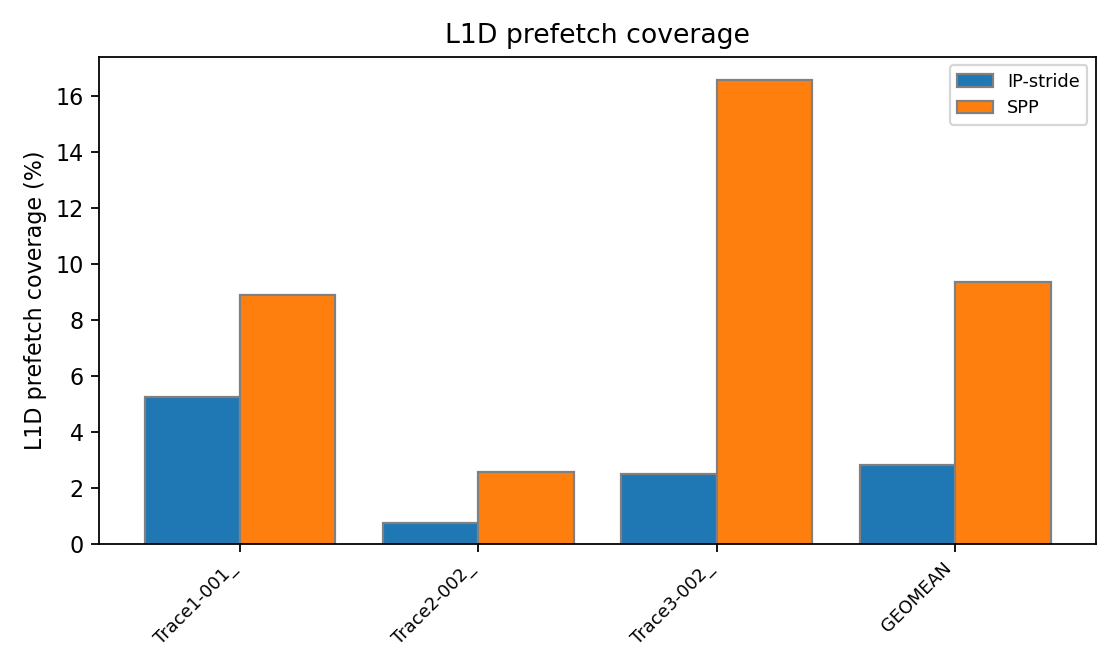
\includegraphics[width=0.8\linewidth]{../plots/task1/coverage.png}
\caption{L1D prefetch coverage.}
\end{figure}\begin{figure}[h]
\centering
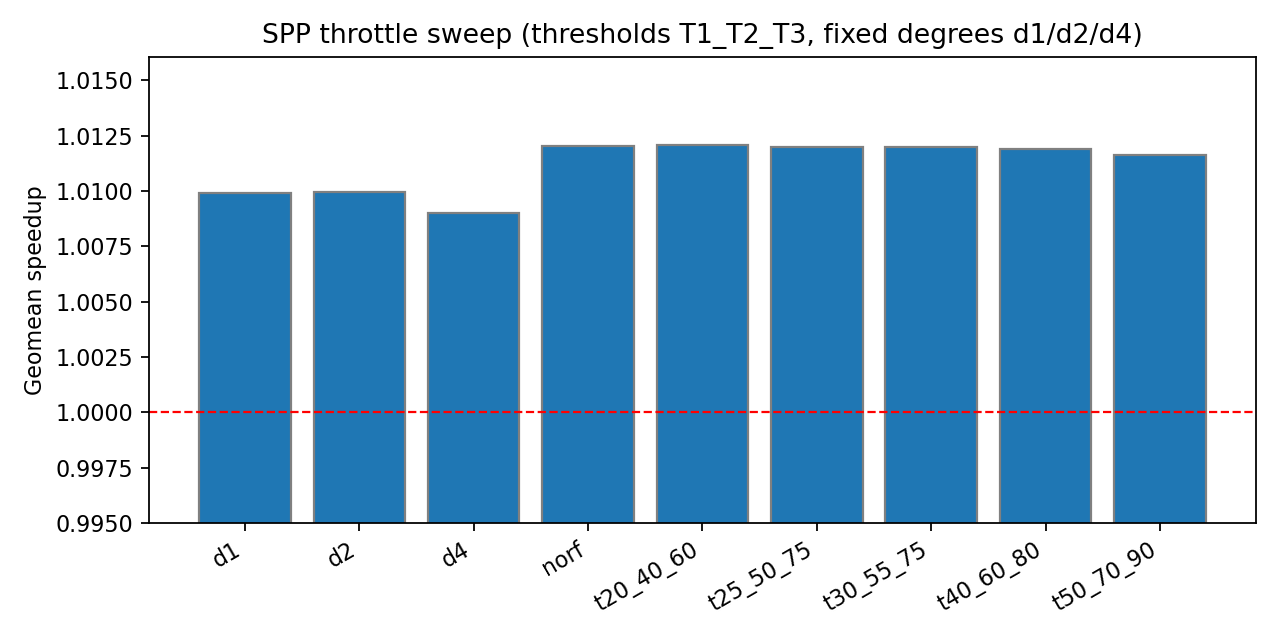
\includegraphics[width=0.8\linewidth]{../plots/task1/sweep.png}
\caption{Throttle sweep: geomean speedup per variant.}
\end{figure}